\documentclass[authoryearcitations]{UoYCSproject}
\usepackage{graphicx}
\graphicspath{ {images/} }
\author{David M. Taylor}
\title{Road Safety Advisory System}
\date{Version 0.2, 2014-March-17}
\supervisor{Dr. Radu Calinescu}
\BEng
\wordcount{xxx}


\abstract{ ... }


\acknowledgements{ ... }

\begin{document}
\maketitle
\listoffigures
\listoftables
\renewcommand*{\lstlistlistingname}{List of Listings}
\lstlistoflistings

\cleardoublepage
\label{sec:start}
\thispagestyle{empty}\cleardoublepage

\chapter{Introduction}

\section{Project Area and Motivation}

It is envisaged that open data, i.e. data that can be freely used and redistributed by anyone, released by governments will lead to major social and economic advances. Deloitte, one of the largest professional services firms in the world, believes that every business should have a strategy to exploit the growing estate of open data \citep{DeloitteAnalytics2012}. Furthermore, in the Open Data Charter of 18 June 2013, it is acknowledged that the use of open data can spur economic growth \citep{CabinetOffice2013}. The Open Data charter states that members of G8 are committed to releasing open data in order to create more accountable, responsive, and effective governments and businesses. Open data increases transparency about what government and businesses are doing, which promotes accountability and good governance.

The Open Data Charter also states that "freely-available government data can be used in innovative ways to create useful tools and products that help people navigate modern life more easily". It is this use of open data that forms the motivation for this project. There are already a large number of applications available that make use of various open data sets. The \textit{data.gov.uk} website has a catalogue of 350+ applications \citep{Data.go}, each of which take open datasets and make the data a usable resource for the general public. 

Several of these applications make use of road safety data published by the UK Department for Transport. These applications all have key limitations that impact the usefulness of the application for the general public and the open data community. For example, they are not capable of highlighting accident hotspots on a user specified route. Additionally, the source code behind these applications isn't open source, so there is little help available for people looking to build their own applications.


\section{Project Aims and Objectives}

The principle aim of this project is to develop and evaluate an application that allows a user to view and interact with open data via an interactive map. More specifically, I aim to build a web application that uses road safety data provided by the UK Department for Transport, in order to warn road users about accident hotspots.

I'm also aiming to build a framework that can be followed by other developers in the future, in order to simplify and encourage the development of similar applications. This will hopefully lead to more open data sets being used for the benefit of the general public.

\section{Statement of Ethics}

All data and technologies used within this project are open source. No human participation is involved so there are no serious ethical concerns.

\section{Report Structure}
The remainder of this report is organised as follows:

Chapter 2 provides a background of open data, and a review of the literature associated with the open data movement. It also covers more general areas of software development, including web application technologies, software engineering methodologies and usability of interactive applications.

Chapter 3 describes the functional and non-functional requirements gathered to develop the road safety advisory system.

Chapter 4 presents the system architecture, development process, technology overview and interface designs. All design decisions made will be explained in this chapter.

Chapter 5 describes the components created and techniques used during the implementation phase. It also describes the testing process followed, and the outcomes of testing.

Chapter 6 provides an evaluation of the application. This includes a discussion of which requirements were met, along with an analysis of the usability, maintainability and limitations of the application.

Chapter 7 summarises the achievements of the project and presents suggestions for future work in this area.

\chapter{Literature Review}

\section{Open Data}

The formal definition of open data states that "open data is data that can be freely used, modified, and shared by anyone for any purpose" \citep{OpenKnowledge}. The release of open datasets by governments is becoming increasingly popular as the benefits become more apparent.

In this section of the report, I will look at the history of the open data movement, benefits and challenges that it introduces, applications using road safety data, and research areas involving open data.

\subsection{The Open Data Movement}

The origins of the open data movement can be traced back as far as 1942, when Robert King Merton explained the importance of making research results freely accessible to all \citep{Chignard2013}. The term open data wasn't coined until 1995, when an American scientific agency used it in reference to a complete and open exchange of scientific information between countries. Researchers were the first to recognise the benefits of sharing data in this manner. This concept of sharing data, along with the growing popularity of open source software led to the foundation of open data.

The open data movement in the UK started to pick up momentum as early as 2006, when The Guardian launched its "Free Our Data" campaign \citep{GuardianTechnology2006}. This campaign called for raw data gathered by Ordnance Survey to be made freely available for reuse by individuals and companies. This campaign partially achieved its goal when, on 1 April 2010, Ordnance Survey released the brand OS OpenData \citep{OrdnanceSurveyteam2010}. The campaign has since continued, with the aim of making more data publicly available. 

In 2007, a meeting was held in Sebastopol, USA, with the aim of defining the concept of open public data and have it adopted by the US presidential candidates. This meeting was hugely successful, and ultimately led to Barack Obama signing two presidential memoranda concerning Open Data the following year. 

In 2009, \textit{data.gov} was launched, with the objective of increasing public access to high value, machine readable datasets. Later in the year, the White House issued an Open Government Directive requiring federal agencies to take immediate, specific steps to achieve key milestones in transparency, participation, and collaboration \citep{Orszag2009}. This required that all agencies post at least three high-value data sets online and register them on \textit{data.gov}.

In 2009, the UK Prime Minister appointed the founder of the World Wide Web, Sir Tim Berners-Lee, as expert advisor on public information delivery \citep{CabinetOffice2009}. Berners-Lee was asked to oversee the work to create a single point of access for government held public data and develop proposals to extend access to data from the wider public sector, including selecting and implementing common standards. This work led to the launch of \textit{data.gov.uk} in January 2010. On launch the site contained 2,500 datasets, and it now contains over 19,500 from areas as diverse as transport, health, and the economy. This increase demonstrates the open data push that has taken place over the last few years in the UK, as the government strives to improve its openness.

The Open Government Partnership was launched in September 2011, with the aim of "securing concrete commitments from governments to promote transparency, empower citizens, fight corruption, and harness new technologies to strengthen governance" \citep{OpenGovernmentPartnership}. From just eight founding governments, there are now 65 participating countries. These countries have made over 1,000 commitments to make their governments more open and accountable.

The Open Data Institute (ODI) was founded by Sir Tim Berners-Lee and Nigel Shadbolt in 2012. The ODI is a not-for-profit organisation, dedicated to promoting Open Data. The ODI aims to "catalyse the evolution of open data culture to create economic, environmental, and social value" \citep{TheOpenDataInstitute}. They now have over 100 members who demonstrate the values of open data to their business and their customers. In the last year, the ODI have trained over 700 people and held over 80 events. They have made considerable effort in promoting the value of open data across the world; there are now 22 'ODI Nodes' in 15 countries \citep{TheOpenDataInstitute2015a}.

On 9 May 2013, Barack Obama signed an executive order \citep{TheWhiteHouse-OfficeofthePressSecretary2013} that made open and machine-readable data the new default for government information. The US government has launched a number of open data initiatives aimed at scaling up open data efforts across the Health, Energy, Climate, Education, Finance, Public Safety, and Global Development sectors. The number of available datasets on \textit{data.gov} has grown rapidly in recent years, with over 130,000 now available. This shows that, like the UK, the US administration has taken large steps to improve its openness.

\subsection{Benefits and Challenges of Using Open Data}


%Tim O'Reilly played a big role in the Sebastopol meeting and the open data movement in the US as a whole. He has since written about how government can improve by embracing open data.  He believes that government can learn from open-source software, by becoming "an open platform that allows people inside and outside government to innovate" \citep{OReilly2011}. 


\subsection{Uses of Road Traffic Data}

Before developing my own application, I will carry out a study of existing web applications that use road safety data. My aim is to identify common characteristics, principles and components that can be reused in my application. I will also look at the limitations of these applications, so that I can look to improve on them.

The applications described below were identified as closest in type and/or purpose to this project.
 
Crash Map \citep{crashmap} displays UK road accidents on an interactive map. You can search for a location, and filter the accident data used according to severity, casualty types, and year of accident (2005-2013). The application plots all accidents found within the current bounding box, with the colour of each marker signifying the severity (see \autoref{fig:crashmap}). If there is a large number of results, you must zoom in further in order for them to be displayed on the map. You can click on a marker for any accident in order to see more information, and then you can request a detailed report for that accident (there is a charge for this service).

The application uses the Google Maps API, but there is no further information about technologies used. The code isn't open source, so there is no benefit to other developers who are looking to build similar applications using open data. 

Crash Map is useful for viewing where accidents have occurred within a specific area, and finding detailed information about them. However, it is reasonable to assume that a user may be more interested in finding out about accidents on a particular route from one location to another, rather than looking at an area. Crash Map is incapable of analysing the data in this way, which is a major limitation.

\begin{figure}
	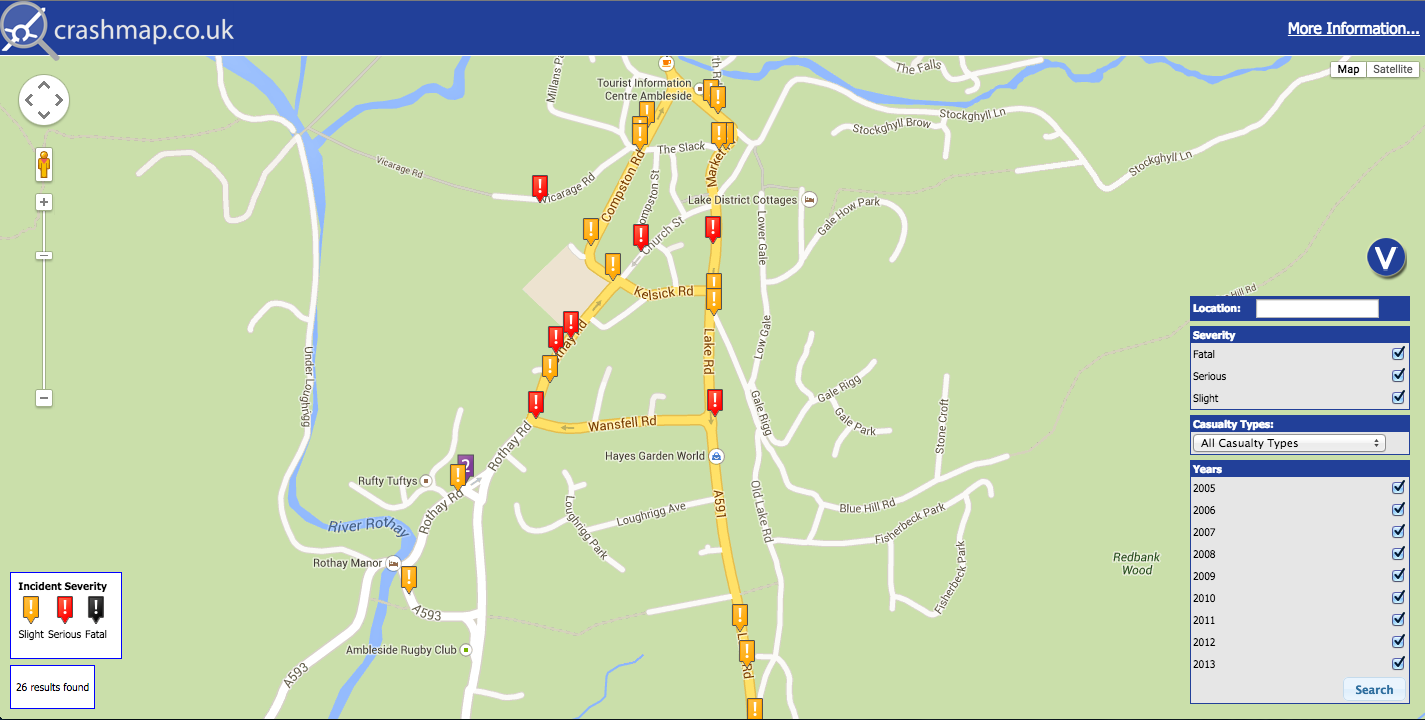
\includegraphics[scale=0.3]{crashmap}
	\caption{Crash Map application}
	\label{fig:crashmap}
\end{figure}

Collision Map \citep{DepartmentforTransport} is similar in purpose to Crash Map. It displays the location of accidents on an interactive map, and also has filters that can be used, including severity, casualty age band and vehicle type (see \autoref{fig:collisionmap}). It differs to Crash Map in that you must select a local highway authority rather than searching for a location or using the map to find it. Clusters of accidents are displayed as one marker on the map, with a number representing how many accidents are in that area. You can reveal the exact location of each accident by zooming in further.

Collision map has several useful features, but has similar limitations to Crash Map. The main advantage of this application is the grouping of accidents to signify hotspots. This makes it very easy to look at an area and see where the most accidents have occurred. A disadvantage in comparison to Crash Map is that you can only use accident data for one year in any search. Like Crash Map, it also lacks the capability of analysing particular routes. This becomes particularly difficult if a route passes through more than one highway authority as you would need to change the search parameters. 

\begin{figure}
	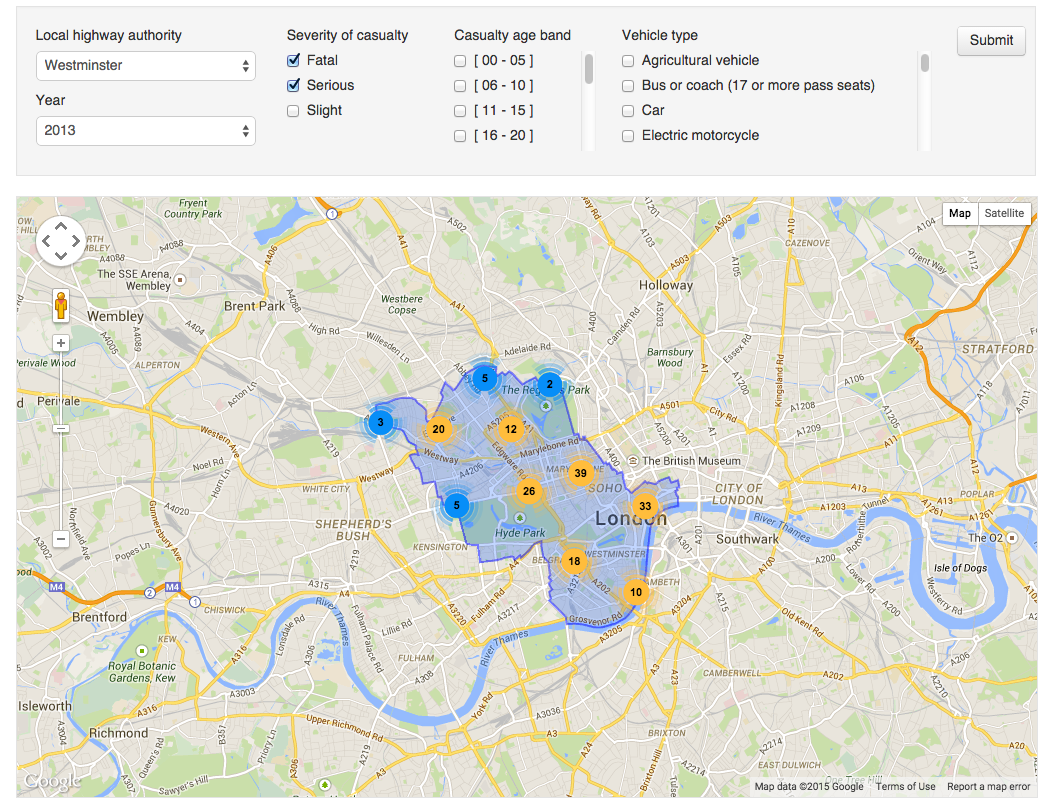
\includegraphics[scale=0.3]{collisionmap}
	\caption{Collision Map application}
	\label{fig:collisionmap}
\end{figure}

Motorcycle Accidents \citep{Mceinsurance} provides an interactive guide to motorcycle accidents in the UK. The aim of this application is to provide motorcyclists with information about where and when it is safest to ride. The application allows you to view statistics about motorcycle accidents on a regional basis (see \autoref{fig:motorcycle}). The application makes use of several fields from the open datasets, including road conditions, time of day and severity. For each field, you can view a break down of the data in each region. For example, you can analyse how accidents depend on time of day in London. The application also presents two key facts for each field in order to summarise the data.

The data is presented in a manner that is easy to analyse for any user, and the facts give a concise summary of the findings from the data. This is adequate to serve the application's purpose, but there are limitations that affect the overall usefulness. For example, it isn't possible to view specific accident hotspots. The regions cover very large areas, and there is no breakdown of where the accidents occur within these areas.

\begin{figure}
	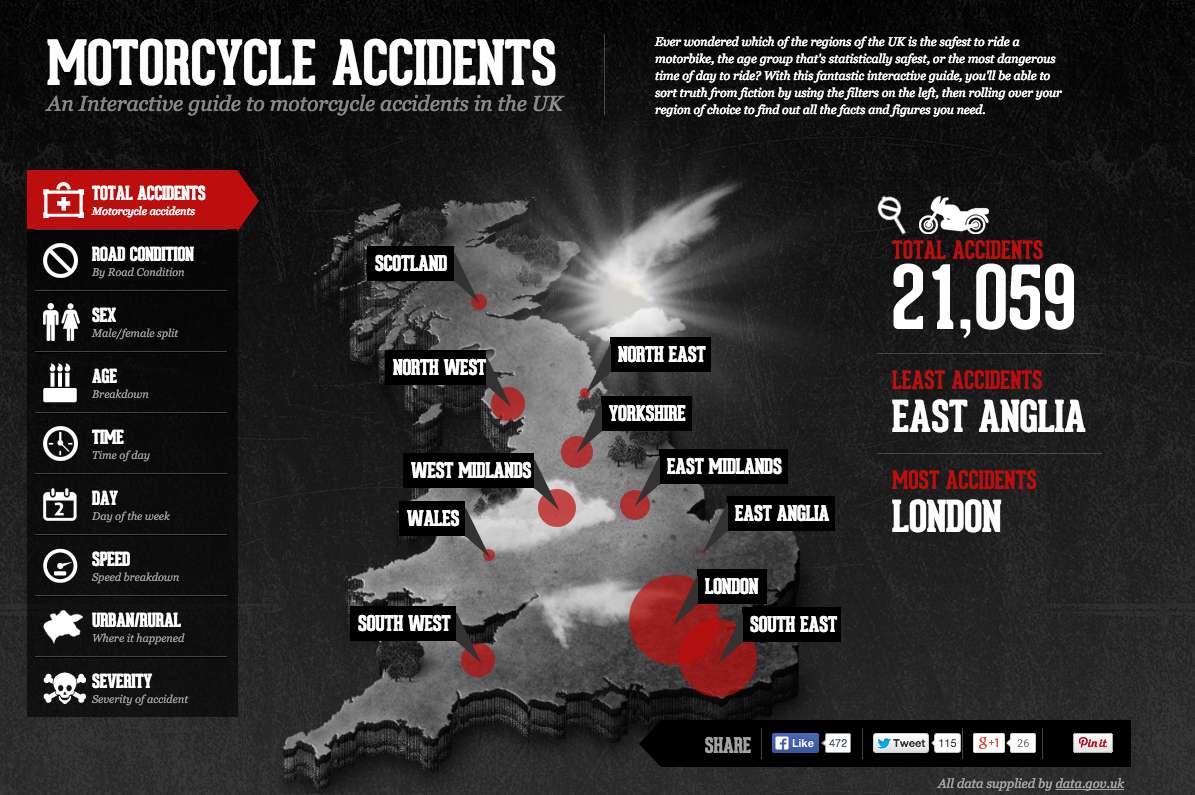
\includegraphics[scale=0.3]{motorcycle}
	\caption{Motorcycle Accidents application}
	\label{fig:motorcycle}
\end{figure}

\subsection{Research in Open Data}

\section{Road Traffic Studies}

\section{Web Application Development}

\section{Software Development Methodologies}

\section{Usability of Interactive Applications}

\chapter{Requirements Analysis}

\section{Functional Requirements}

\begin{tabular}{| p{2.2cm} | p{7.5cm} | p{2cm} |}
	\hline
	\textbf{Requirement ID} & \textbf{Description} & \textbf{Importance} \\ \hline
	FR1 & The application should use road safety data published by the UK Department for Transport to warn users about accident hotspots. & High \\ \hline
	FR2 & Users should be able to specify road journeys, and the road safety data should be used to highlight risks on the selected route. & High \\ \hline
	FR3 & Users should be able to specify time of travel in order to further filter the data. & Medium \\ \hline
	FR4 & Users should be able to set warning thresholds, such as frequency and severity of accidents. & Medium \\ \hline
	FR5 & Users should be able to specify weather conditions in order to further filter the data. & Low \\ \hline
	FR6 & Weather data should be retrieved from the Met Office DataPoint service using the location and time parameters specified by the user. This data should then be used to filter the road safety data. & Low \\ \hline
	FR7 & The application should suggest lower risk routes for the specified journey. & Low \\ \hline
	FR8 & The location of incidents should be displayed on an interactive map. & High \\ \hline
	FR9 & Users should be able to retrieve additional information about an incident. & Medium \\ \hline
	FR10 & UThe application should be compatible with the latest versions of Google Chrome, Mozilla Firefox and Internet Explorer. & High \\ \hline
	FR11 & The application should be compatible with mobile devices. & Low \\ \hline
	FR12 & The site administrator should be able to add and remove datasets through a user-friendly GUI. & High \\ \hline
	FR13 & The road safety data should be automatically updated when new datasets are released. & Low \\ \hline
	FR14 & A generic ‘boilerplate’ implementation should be developed that can be reused to develop other Open Data applications. & Medium \\
	\hline
\end{tabular}

\section{Non-functional Requirements}

\begin{tabular}{| p{2.2cm} | p{7.5cm} | p{2cm} |}
	\hline
	\textbf{Requirement ID} & \textbf{Description} & \textbf{Importance} \\ \hline
	NFR1 & The results of any data analysis should be presented in a user-friendly way. & High \\ \hline
	NFR2 & The response time of the application should be <5 seconds, assuming that the user's connection isn't the bottleneck. & High \\ \hline
	NFR3 & The user interface should use standard controls. & Medium \\
	\hline
\end{tabular}


\chapter{Design}

\section{System Architecture}

\subsection{LAMP}

\subsection{UML Diagram}

\section{Development Process}

\section{Technology Overview}

\subsection{PHP}

\subsection{MySQL}

\subsection{Google Maps API}

\subsection{Version Control System}

\section{Interface Design}

\subsection{Wireframes}

\section{Summary}

\chapter{Implementation and Testing}

\section{Components}

\section{Techniques}

\section{Testing}

\section{Summary}

\chapter{Evaluation}

\section{Discussion}

\section{Usability}

\section{Maintainability}

\section{Limitations}

\chapter{Conclusions}

\section{Lessons Learnt}

\section{Future Work}


\bibliography{library}


\end{document}
